\documentclass[floatfix,nofootinbib,superscriptaddress,fleqn,preprint]{revtex4-2}  
%\documentclass[aps,epsfig,tightlines,fleqn]{revtex4}
\usepackage[utf]{kotex}
\usepackage[HWP]{dhucs-interword}
\usepackage[dvips]{color}
\usepackage{graphicx}
\usepackage{bm}
%\usepackage{fancyhdr}
%\usepackage{dcolumn}
\usepackage{defcolor}
\usepackage{amsmath}
\usepackage{amsfonts}
\usepackage{amssymb}
\usepackage{amscd}
\usepackage{amsthm}
\usepackage[utf8]{inputenc}
 \usepackage{setspace}
%\pagestyle{fancy}

\begin{document}

\title{\Large 2022년 1학기 물리학 I: Quiz 21}
\author{김현철\footnote{Office: 5S-436D (면담시간 매주
    화요일-16:00$\sim$20:00)}} 
\email{hchkim@inha.ac.kr}
\affiliation{Hadron Theory Group, Department of Physics,
Inha University, Incheon 22212, Republic of Korea }
\date{Spring semester, 2022}


\vspace{1.cm}
\begin{abstract}
\noindent \textbf{ {\color{red}주의}: \color{blue} 단 한 번의
  부정행위도 절대 용납하지 않습니다. 적발 시, 학점은 F를 받게 됨은
  물론이고, 징계위원회에 회부합니다. One strike out임을 명심하세요.}\\
\\
문제는 다음 쪽부터 나옵니다.  \\ \\
{\bf Date:} 2022년 5월 25일 (수) 15:30-16:15
\\
{\bf 학번:} \hspace{4cm}
{\bf 이름:} 

\end{abstract}
\maketitle

\newpage
\noindent {\bf 문제 1. (100 pt)} 
103.0 kPa의 계기압력에서
$0.140\,\mathrm{m}^3$의 부피를 갖는 101.3 kPa의 압력까지 등온 팽창한
다음, 일정압력에서 처음부피가 될 때까지 냉각시켰다. 기체가 한 일을
계산하여라(계기압력은 실제압력과 대기압의 차이이다). 
 \newpage

{\color{gray} [문제 풀이 쪽]}

\newpage

\noindent {\bf 문제 2. (100 pt)}
$\gamma=1.30$인 기체가 처음 상태 273 
K, 1.00 atm에서 갑자기 처음부피의 절반으로 단열압축되었다.
\begin{itemize}
\item[(가)] 나중 압력과
\item[(나)] 나중 온도를 구하여라. 
\item[(다)] 그런 다음 기체가 일정한 압력에서 273 K까지 냉각되었다면,
  나중부피는 얼마인가?   
\end{itemize}
\newpage
{\color{gray} [문제 풀이 쪽]}

\newpage

\noindent {\bf 문제 3. (200pt)}
그림~\ref{fig:1}은 1.00 몰의 단원자
이상적인 기체의 순환과정이다.  각각의 과정에서 온도는 $T_1=400$ K,
$T_2=600$ K, $T_3=455$ K이다.  $1\to 2$ 과정에 대해
\begin{figure}[ht]
  \centering
  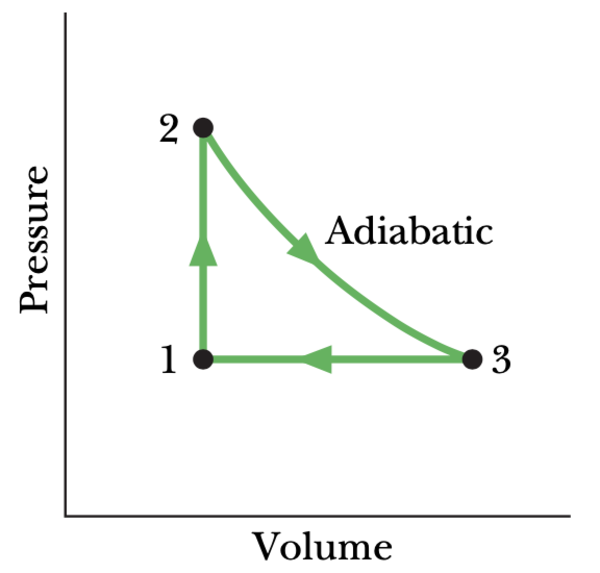
\includegraphics[scale=0.6]{Qfig23-1.pdf}
  \caption{문제 3}
  \label{fig:1}
\end{figure}
\begin{itemize}
\item[(가)] 열 $Q$
\item[(나)] 내부에너지 변화 $\Delta U$
\item[(다)] 한 일은 각각 얼마인가? 
\item[(라)] $2\to 3$과정에 대하여 $Q$
\item[(마)] $\Delta U$
\item[(바)] $W$는 각각 얼마인가? 
\item[(사)] $3\to 1$과정에서 
\item[(아)] $Q$
\item[(자)] $\Delta U$
\item[(차)] $W$는 얼마인가?
\item[(카)] 전체 순환 과정에 대해 $Q$
\item[(타)] $\Delta U$
\item[(파)] $W$는 각각 얼마인가?
\end{itemize}
점 1에서 처음 압력은 1.00 기압 ($=1.013\times 10^5$ Pa)이다. 점 2에서
\begin{itemize}
\item[(하)] 부피 
\item[(거)] 압력을 구하여라. 
\end{itemize}
점 3에서 
\begin{itemize}
\item[(너)] 부피 
\item[(더)] 압력을 구하여라. 
\end{itemize}
\newpage
{\color{gray} [문제 풀이 쪽]}

\newpage

\end{document}